\documentclass[border=5pt]{standalone}

\usepackage[utf8]{inputenc}
\usepackage{garamondx}

\usepackage[x11names]{xcolor}
\usepackage{tikz}
\usetikzlibrary{shapes.geometric, arrows, positioning}

\definecolor{darkolivegreen}{rgb}{0.33, 0.42, 0.18}
\definecolor{darkbyzantium}{rgb}{0.36, 0.22, 0.33}
\definecolor{darkelectricblue}{rgb}{0.33, 0.41, 0.47}

\tikzstyle{stage}=[rectangle, rounded corners, minimum width=15em, minimum height=2em, text centered, draw=black, fill=darkolivegreen!30, text width=15em]
\tikzstyle{additional}=[rectangle, rounded corners, minimum width=15em, minimum height=2em, text centered, draw=black, text width=15em]
\tikzstyle{detail} = [rectangle, rounded corners, minimum width=15em, minimum height=2em, text centered, draw=black, fill=darkbyzantium!30, text width=15em]
\tikzstyle{branch}=[rectangle, rounded corners, minimum width=15em, minimum height=2em, text centered, draw=black, fill=darkelectricblue!30, text width=15em]
\tikzstyle{arrow}=[very thick, ->,>=latex]

% Based on:
%   https://gist.github.com/jakewilliami/5be1e7ac454ba7b015d2737359bc83ed
\begin{document}
	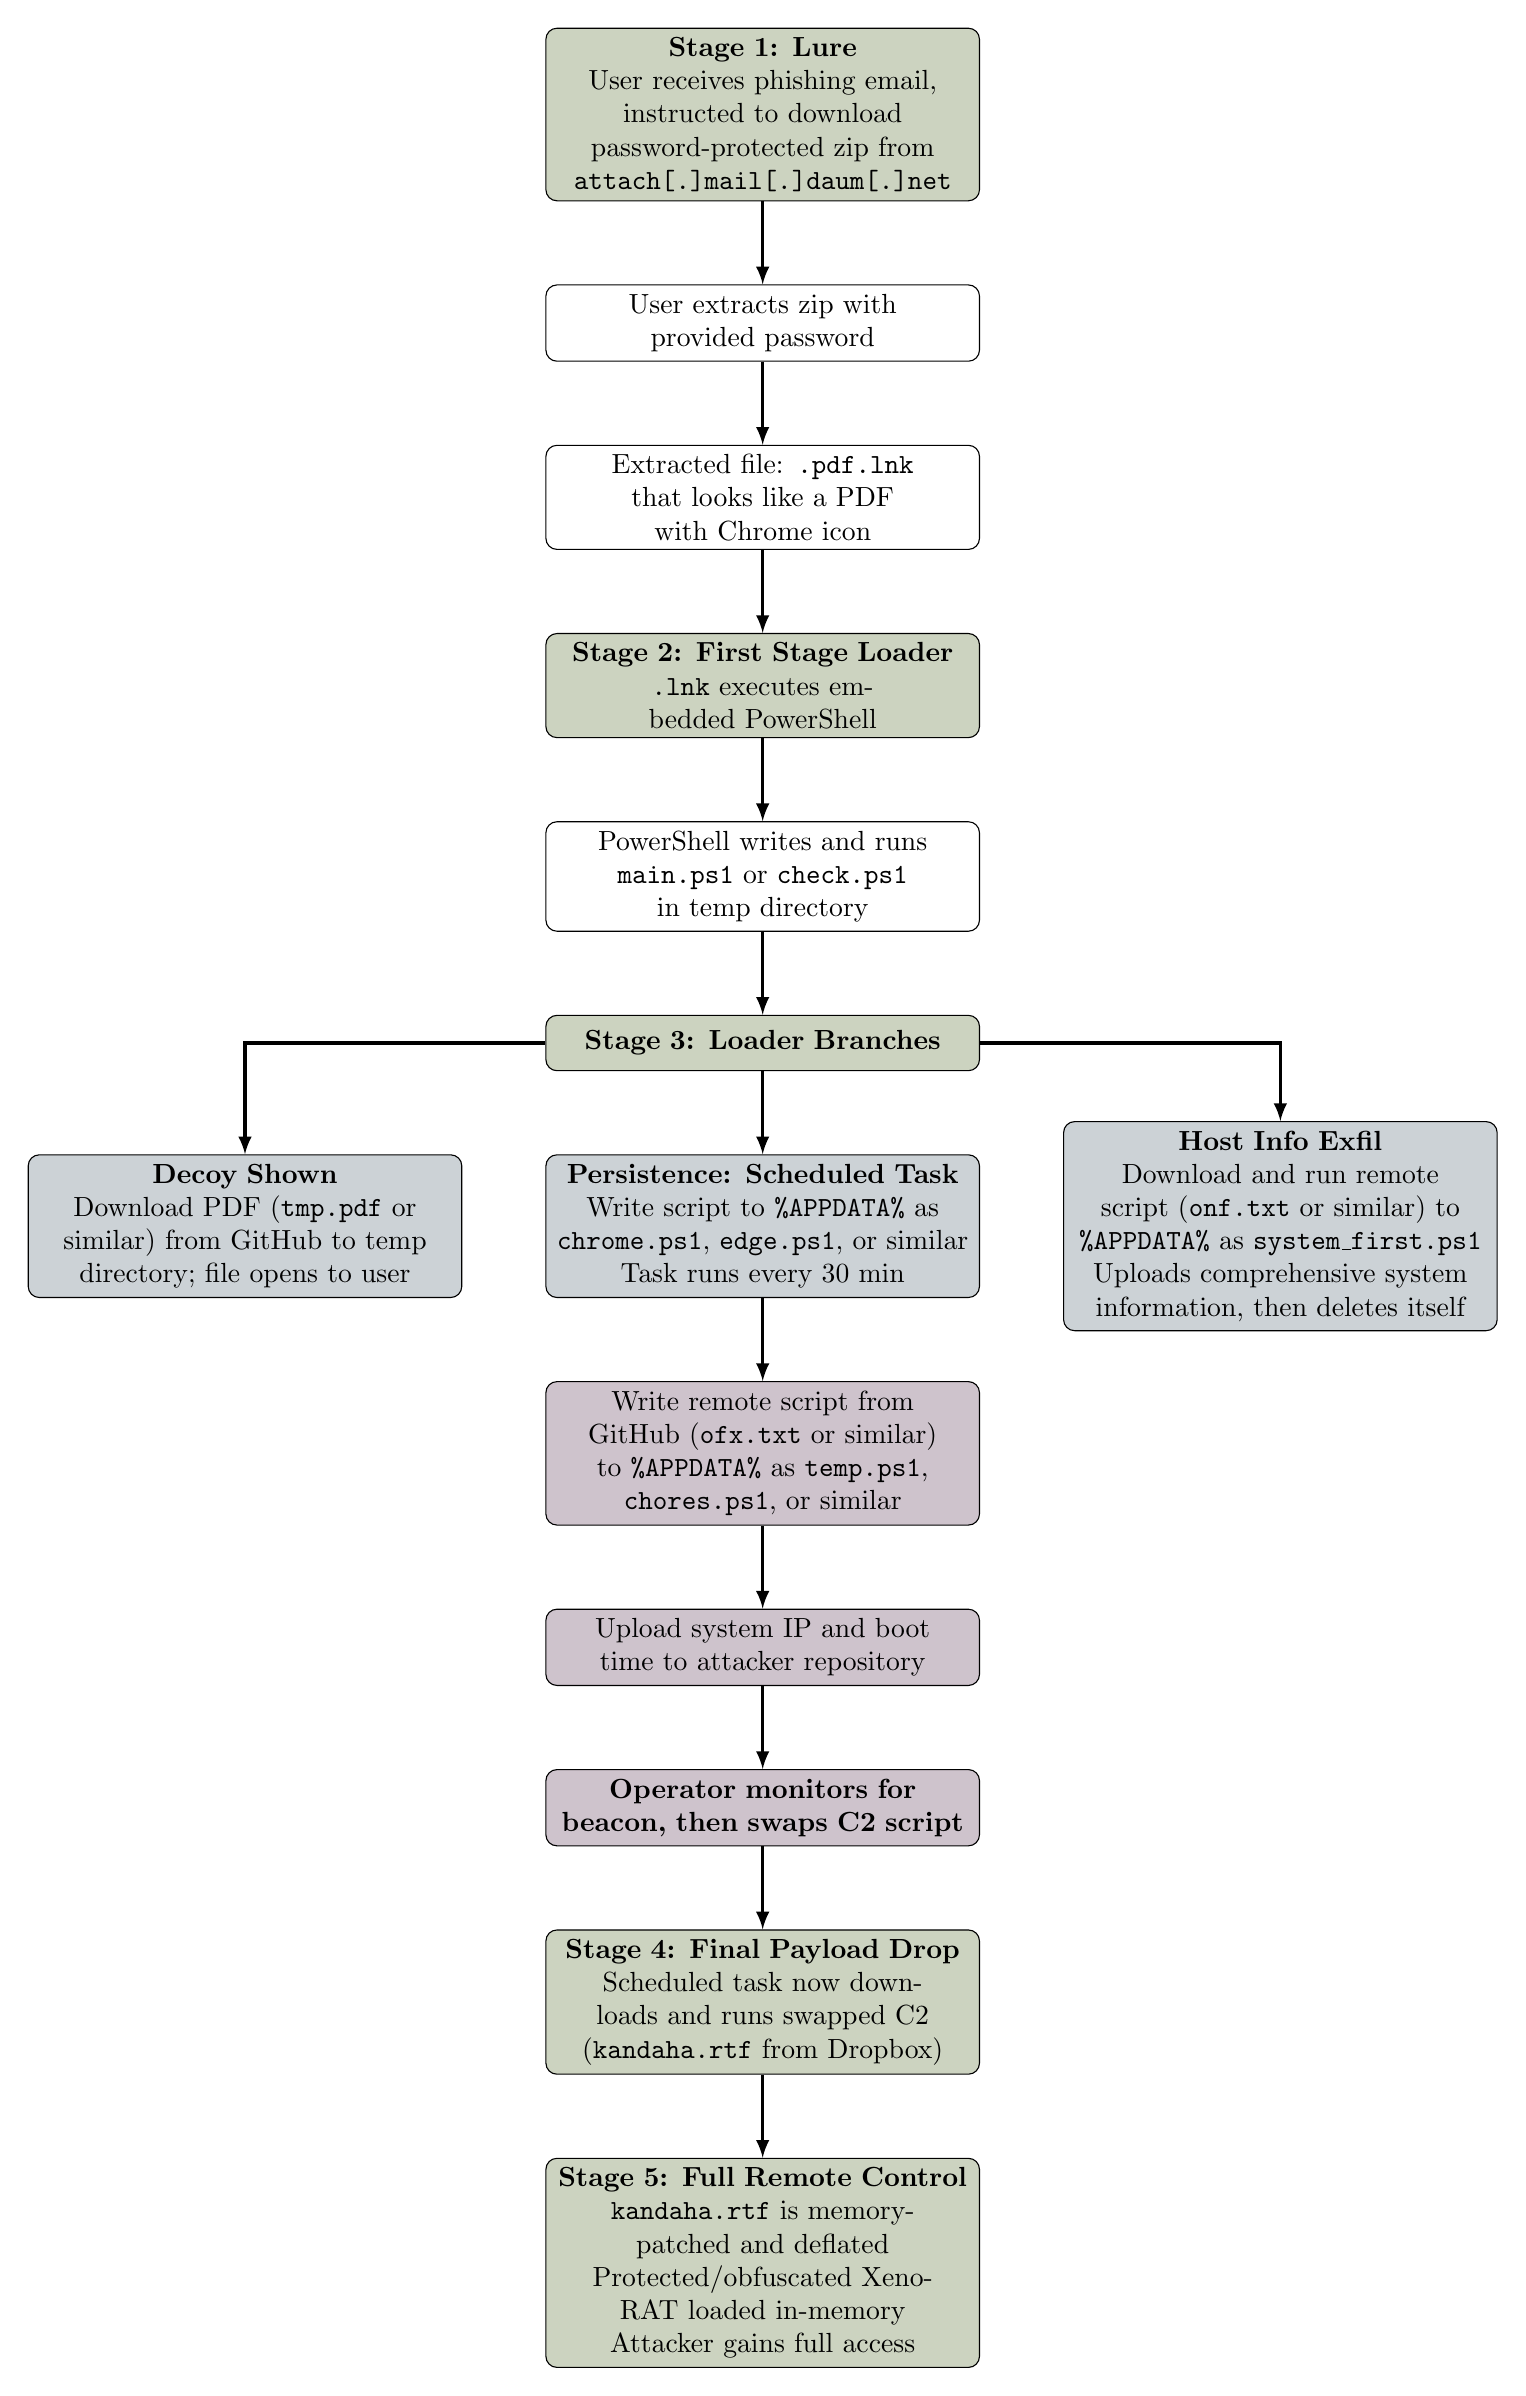
\begin{tikzpicture}[node distance=3em]
		\node (lure) [stage] {\textbf{Stage 1: Lure}\\User receives phishing email, instructed to download password-protected zip from \texttt{attach[.]mail[.]daum[.]net}};
		\node (zip) [additional, below=of lure] {User extracts zip with provided password};
		\node (lnk) [additional, below=of zip] {Extracted file: \texttt{.pdf.lnk} that looks like a PDF with Chrome icon};
		
		\node (stage2) [stage, below=of lnk] {\textbf{Stage 2: First Stage Loader}\\\texttt{.lnk} executes embedded PowerShell};
		\node (mainps1) [additional, below=of stage2] {PowerShell writes and runs \texttt{main.ps1} or \texttt{check.ps1} in temp directory};
		
		\node (stage3) [stage, below=of mainps1] {\textbf{Stage 3: Loader Branches}};
		
		\node (persistence) [branch, below=of stage3] {\textbf{Persistence: Scheduled Task}\\Write script to \texttt{\%APPDATA\%} as \texttt{chrome.ps1}, \texttt{edge.ps1}, or similar\\Task runs every 30 min};
		\node (decoy) [branch, left=of persistence] {\textbf{Decoy Shown}\\Download PDF (\texttt{tmp.pdf} or similar) from GitHub to temp directory; file opens to user};
		\node (recon) [branch, right=of persistence] {\textbf{Host Info Exfil}\\Download and run remote script (\texttt{onf.txt} or similar) to \texttt{\%APPDATA\%} as \texttt{system\_first.ps1}\\Uploads comprehensive system information, then deletes itself};
		
		\node (tempps1) [detail, below=of persistence] {Write remote script from GitHub (\texttt{ofx.txt} or similar) to \texttt{\%APPDATA\%} as \texttt{temp.ps1}, \texttt{chores.ps1}, or similar};
		\node (beacon) [detail, below=of tempps1] {Upload system IP and boot time to attacker repository};
		\node (swap) [detail, below=of beacon] {\textbf{Operator monitors for beacon, then swaps C2 script}};
		
		\node (stage4) [stage, below=of swap] {\textbf{Stage 4: Final Payload Drop}\\Scheduled task now downloads and runs swapped C2 (\texttt{kandaha.rtf} from Dropbox)};
		\node (stage5) [stage, below=of stage4] {\textbf{Stage 5: Full Remote Control}\\\texttt{kandaha.rtf} is memory-patched and deflated\\Protected/obfuscated XenoRAT loaded in-memory\\Attacker gains full access};
						
		\draw [arrow] (lure) -- (zip);
		\draw [arrow] (zip) -- (lnk);
		\draw [arrow] (lnk) -- (stage2);
		\draw [arrow] (stage2) -- (mainps1);
		\draw [arrow] (mainps1) -- (stage3);
		\draw [arrow] (stage3) -- (persistence);
		\draw [arrow] (stage3) -| (decoy);
		\draw [arrow] (stage3) -| (recon);
		\draw [arrow] (persistence) -- (tempps1);
		\draw [arrow] (tempps1) -- (beacon);
		\draw [arrow] (beacon) -- (swap);
		\draw [arrow] (swap) -- (stage4);
		\draw [arrow] (stage4) -- (stage5);
	\end{tikzpicture}
\end{document}
